\documentclass{article}
% \documentclass[12pt,a4paper,oneside,fleqn]{book}
% \usepackage[slovene]{babel}
\usepackage[english]{babel}

\usepackage[a4paper,top=2cm,bottom=2cm,left=3cm,right=3cm,marginparwidth=1.75cm]{geometry}
% \usepackage[left=30mm,
% right=25mm,
% top=30mm,
% bottom=25mm]{geometry}

\usepackage{biblatex}
\addbibresource{reffrenc.bib}

\usepackage{lipsum}
\usepackage{array}
\usepackage{caption}
\usepackage{amsmath}
\usepackage{graphicx}
\usepackage{subcaption}
\usepackage[colorlinks=true, allcolors=blue]{hyperref}
\usepackage[nodisplayskipstretch]{setspace}

\usepackage{listings}
\usepackage{xcolor}

\definecolor{codegreen}{rgb}{0,0.6,0}
\definecolor{codegray}{rgb}{0.5,0.5,0.5}
\definecolor{codepurple}{rgb}{0.58,0,0.82}
\definecolor{backcolour}{rgb}{0.95,0.95,0.92}

\lstdefinestyle{codestyle}{
    backgroundcolor=\color{backcolour},   
    commentstyle=\color{codegreen},
    keywordstyle=\color{magenta},
    numberstyle=\tiny\color{codegray},
    stringstyle=\color{codepurple},
    basicstyle=\ttfamily\footnotesize,
    breakatwhitespace=false,         
    breaklines=true,                 
    captionpos=b,                    
    keepspaces=true,                 
    % numbers=left,   
    numbers=none,
    numbersep=5pt,                  
    showspaces=false,                
    showstringspaces=false,
    showtabs=false,                  
    tabsize=2
}

\lstset{style=codestyle}


\title{OracleDepth Phase1}
\author{Kristijan Danov 23221364}
\date{}

\begin{document}

\maketitle

\tableofcontents
\newpage

\section{Introduction}
    In this report we will go over the basic theory behind the pinhole camera model, ChArUco markers and camera calibration. We will also use python code to perform camera calibration and undistort images. And we will perform 3D reconstruction in Meshroom 2023.3.0. For the code we will use Python 3.11 and the following modules: 
\begin{itemize}
    \item numpy==1.24.2
    \item opencv\_contrib\_python==4.11.0.86
\end{itemize}

\section{Theory}
    In order to understand what we are doing with our code firstly we must have a good base in theory. Here we will go over some basics on pinhole cameras, camera parameters, distortion, camera calibrations and etc. 

\subsection{Pinhole camera model}
    The pinhole camera model is an ideal description of the mathematical relationship between the real 3D space and the 2D image projection. The pinhole camera is made up of a pinhole and an image plane. Because the pinhole is in between the image plane and the 3D world, any ray emitted from the 3D world has to pass through the pinhole before reaching the image plane. In this case the projected image is inverted.(\ref{fig:obscura}a) This natural phenomenon is called camera obscura and has been used through history being described by Ibn al-Haytham in the 10th century. If we place a plane in front of the pinhole, then the projected image won't be inverted.(\ref{fig:obscura}b) 

\begin{figure}[h]
    \centering
    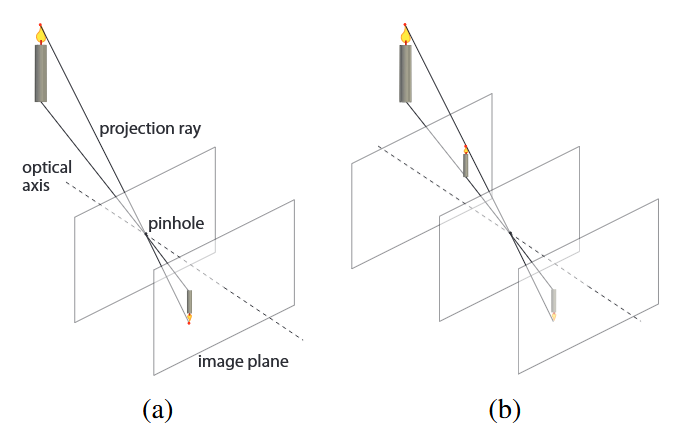
\includegraphics[width=0.5\linewidth]{imgs/obscura.png}
    \caption{Pinhole camera model}
    \label{fig:obscura}
\end{figure}

To mathematically understand this model, first we need to define 2 coordinate systems of interest. Those are:
\begin{itemize}
    \item The external coordinate system('W' for 'world') defined by center $\pmb{O_W}$ and axes $[X_W, Y_W, Z_W]$
    \item The camera coordinate system('C' for 'camera') defined by center $\pmb{O_C}$ and axes $[X_C, Y_C, Z_C]$
\end{itemize}



\begin{figure}[h]
    \centering
    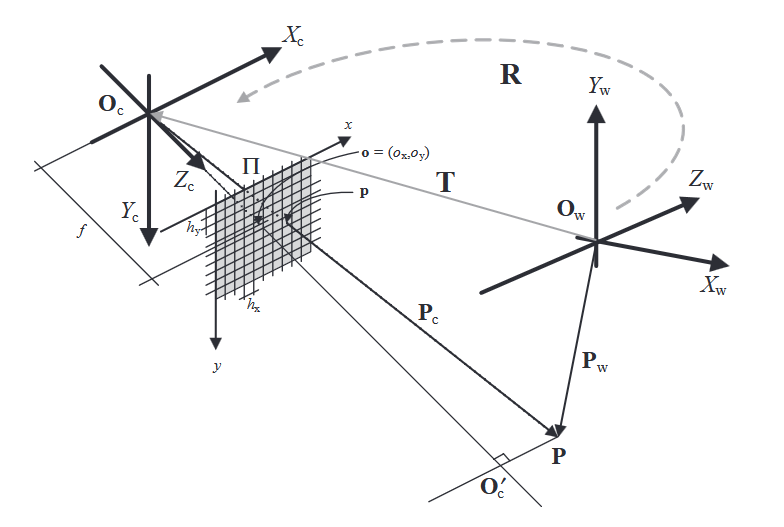
\includegraphics[width=0.8\linewidth]{imgs/pinholemodel.png}
    \caption{Pinhole camera model coordinate systems and points}
    \label{fig:pinhole}
\end{figure}

These 2 coordinate systems are related by translation $\pmb{T}$ and rotation $\pmb{R}$. \\
The following points can be seen on figure \ref{fig:pinhole}. \\
The image plane $\pmb{\Pi}$ is tessellated into rectangles called pixels. Pixels in a camera form discrete photosensing locations that sample any image projected onto the plane. Each pixel is indexed by a pair of coordinates expressed by natural numbers. $h_x$ and $h_y$ determine the physical dimensions of a single pixel. \\
Point $\pmb{O_C}$ called the focal point. Its projection onto $\pmb{\Pi}$ in $Z_C$ direction determines the principal point $o$ on the image plane. The distance from focal point $\pmb{O_C}$ to the principal point $o$ is called the focal length $f$. $Z_C$ is also called the principal axis. $\pmb{O_C}$, $o$ and $\pmb{O_C'}$ lie on it.  \\
We can define some point $\pmb{P}$ in the real world and its position is given by the chosen coordinate system, $\pmb{P_C}$ for the camera coordinate system or $\pmb{P_W}$ for the external coordinate system. \\
Point $\pmb{p}$ is an image of point $\pmb{P}$ onto the image plane with a center point $\pmb{O_C}$. We can define their coordinates as: 
\[
    \pmb{P} = [X, Y, Z]^T  \qquad \pmb{p} = [x, y, z]^T
\]


Because we have similar triangles $\triangle\pmb{O_C p o}$ and $\triangle\pmb{O_C P O_C'}$ we obtain:
\[
    x=f\frac{X}{Z} \qquad y=f\frac{Y}{Z} \qquad z =f
\]
The pinhole camera model can be defined by 2 sets of parameters:
\begin{itemize}
    \item Extrinsic parameters
    \item Intrinsic parameters
\end{itemize}

    \subsubsection{Extrinsic parameters}
        Extrinsic parameters are all the geometric parameters that are needed for the change from the camera coordinate system to the external coordinate system. This change is described by translation $\pmb{T}$ and rotation $\pmb{R}$. We can write the change of point $\pmb{P}$ related by world coordinates as $\pmb{P_W}$ to camera coordinates $\pmb{P_C}$ as:
\[
    \pmb{P_C} = \pmb{R}(\pmb{P_W}-\pmb{T})
\]
The extrinsic parameters $\pmb{T}$ and $\pmb{R}$ are written as:
\[
    \pmb{T} = \pmb{O_W} - \pmb{O_C} = \begin{bmatrix}
                                        T_1 \\
                                        T_2 \\
                                        T_3
                                        \end{bmatrix}_{3\times3}
                                        \qquad
    \pmb{R} =
    \begin{bmatrix}
        \pmb{R_{1}} \\
        \pmb{R_{2}} \\
        \pmb{R_{3}} \\
    \end{bmatrix}_{3\times3}
    = \begin{bmatrix}
        R_{11} & R_{12} & R_{13} \\
        R_{21} & R_{22} & R_{23} \\
        R_{31} & R_{32} & R_{33} \\
    \end{bmatrix}_{3\times3}
\]
We can write these extrinsic parameters as matrix $\pmb{M_e}$

\[
    \pmb{M_e} = 
    \begin{bmatrix}
        \pmb{R_1} & -\pmb{R_1 T} \\
        \pmb{R_2} & -\pmb{R_2 T} \\
        \pmb{R_3} & -\pmb{R_3 T} \\        
    \end{bmatrix}_{3\times4}
\]
    
    \subsubsection{Intrinsic parameters}
        Intrinsic parameters are the focal length $f$ and parameters that map the camera coordinate system onto the image plane(also distortion parameters are here, but for now we will disregard them). \\
We can write these intrinsic parameters as matrix $\pmb{M_i}$
\[
    \pmb{M_i} = 
    \begin{bmatrix}
        \frac{f}{h_x} & 0 & o_x \\
        0 & \frac{f}{h_y} & o_y \\
        0 & 0 & 1
    \end{bmatrix}_{3\times3}
\]

\subsection{Projective transformation}
    The mapping of point $\pmb{P}$ to $\pmb{p}$ on the image plane is performed by transformation $\pmb{M}$
\[
    \pmb{p} = \pmb{M P}
\]
Matrix $\pmb{M}$ is called the projection matrix and is made up of the intrinsic and extrinsic parameter matrices.
\[
    \pmb{M} = \pmb{M_i M_e}
\]


\subsection{Distortion}
    In the real world pinhole cameras aren't practical because, if the pinhole is large the image is blurred and if it's small the image is dim. For this reason we use lenses which refocus incoming rays onto the image plane. Because of the use of lenses, distortion occurs. Here we will go over radial and tangential distortion. \\
Let $(x, y)$ be the coordinates of a point on the undistorted image and $(x_d, y_d)$ the coordinates of that same point on the distorted image. \\

Radial distortion the "barrel" or "fish-eye" effect that occurs in images. We can represent radial distortion as
\begin{gather}
    x_d = x(1 + k_1 r^2 + k_2 r^4 + k_3 r^6) \notag\\
    y_d = y(1 + k_1 r^2 + k_2 r^4 + k_3 r^6) \notag\\
    r^2 = x^2+y^2
    \label{radialdistEq}
\end{gather}

\begin{figure}[h]
    \centering
    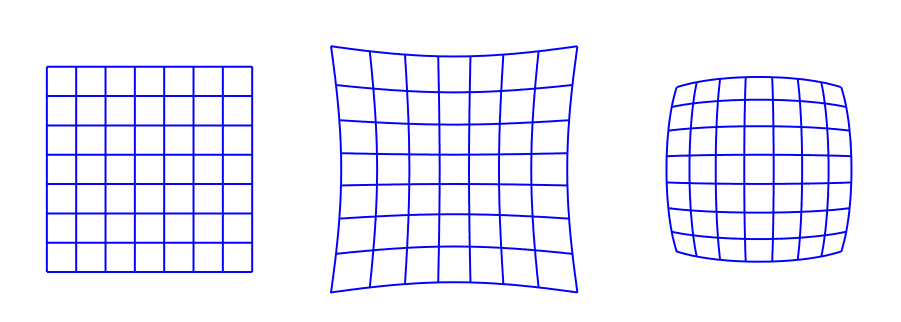
\includegraphics[width=0.5\linewidth]{imgs/radialdist.png}
    \caption{Radial distortion}
    \label{fig:raddist}
\end{figure}

Tangential distortion occurs because the lenses are not perfectly parallel to the imaging plane and it can be represented as

\begin{gather}
    x_d = x+[2p_1xy+p_2(r^2+2x^2)] \notag\\
    y_d = y+[p_1(r^2+2y^2)+2p_2xy]
    \label{tangentialdistEq}
\end{gather}

To find out the distortion coefficients $(k_1, k_2, p_1, p_2, p_3)$ and the intrinsic and extrinsic parameters we perform camera calibration. 

\subsection{Camera calibration}
    Camera calibration is the process of finding out the intrinsic, extrinsic parameters and the distortion coefficients. One of their uses is removing distortion. \\
Calibration is based on solving basic geometrical equations based on a chosen calibrating object. We detect the corners of the pattern. Most common are ChArUco patterns. ChArUco patterns are made up of chessboard and ArUco patterns. ArUco markers have fast detection but their accuracy is not high. Chessboards have a greater accuracy because each corner is surrounded by two black squares but the it has to be completely visible and its harder to detect. By combining these two we get the best of both of them. With the ArUco markers we can interpolate the positions of chessboard corners which allows partial views. Also because of the ArUco markers, each chessboard corner can have a unique id not dependent on if the pattern is rotated. 

\begin{figure}[h]
    \begin{subfigure}{.5\textwidth}
        \centering
        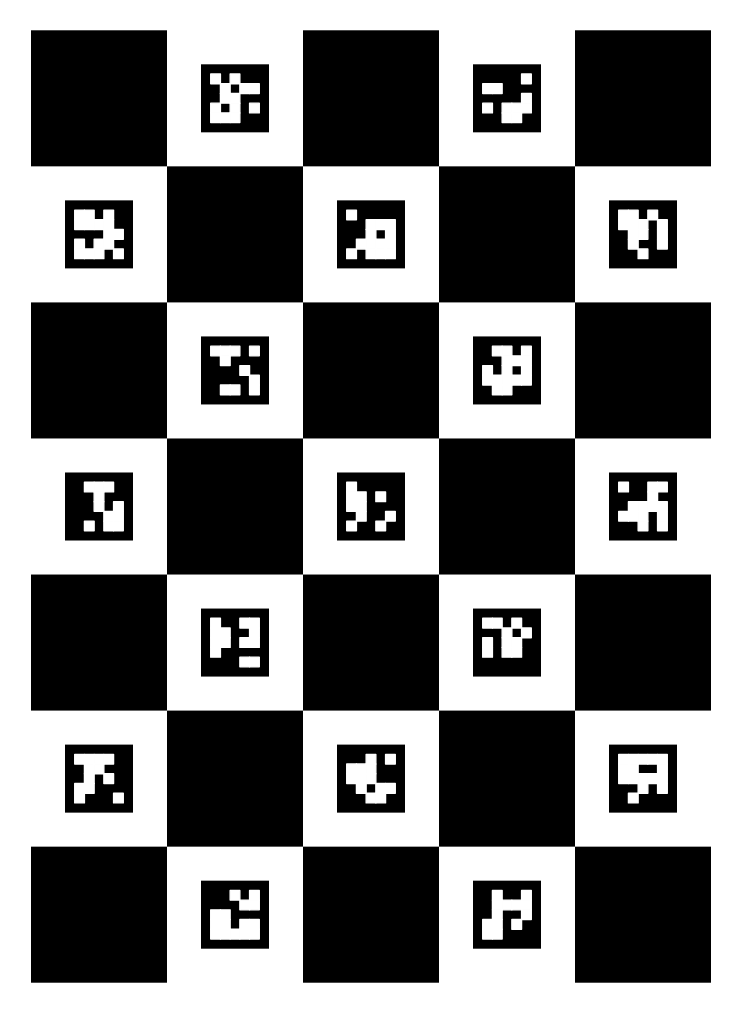
\includegraphics[width=.95\linewidth]{imgs/charuco.png}
        \caption{Example board}
    \end{subfigure}
    \begin{subfigure}{.5\textwidth}
        \centering
        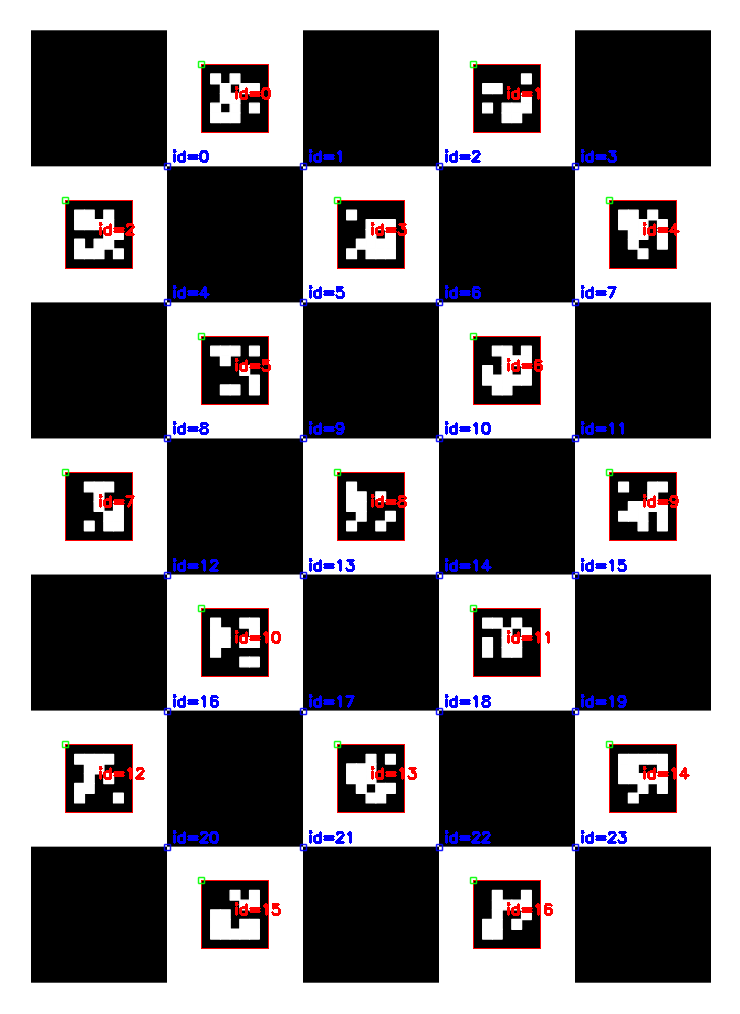
\includegraphics[width=.95\linewidth]{imgs/charucoDetect.png}
        \caption{Board with detected markers and corners drawn}
    \end{subfigure}
    \caption{ChArUco boards}
\end{figure}

\subsubsection{Zhang method for computing the intrinsic parameters}
In this subsection we will go over the math in the Zhang method for camera calibration[ref]. \\

Lets start with writing the equation correlating the 3D point to the 2D image point. The left and right matrices are the intrinsic and extrinsic matrix accordingly. The intrinsic matrix is written a bit differently than before, that's because here are we take account of skewness and aspect ratio. 
\[
    \begin{bmatrix}
    x \\
    y \\
    1 
    \end{bmatrix}
    =
    \begin{bmatrix}
    c   &   cs  &   x_H \\
    0   &   c(1+m)  &   y_H \\
    0   &   0   &   1 
    \end{bmatrix}
    \begin{bmatrix}
    r_{11}   &   r_{12}  &  r_{13}  &   t_1 \\
    r_{21}   &   r_{22}  &  r_{23}  &   t_2 \\
    r_{31}   &   r_{32}  &  r_{33}  &   t_3
    \end{bmatrix}
    \begin{bmatrix}
        X \\
        Y \\
        Z \\
        1
    \end{bmatrix}
\]
By assuming Z=0(when we use boards, all the points on the boards have the same Z=0 value) we can eliminate the 3rd column of the extrinsic matrix. 
\begin{equation}
    \begin{bmatrix}
    x \\
    y \\
    1 
    \end{bmatrix}
    =
    \begin{bmatrix}
    c   &   cs  &   x_H \\
    0   &   c(1+m)  &   y_H \\
    0   &   0   &   1 
    \end{bmatrix}
    \begin{bmatrix}
    r_{11}   &   r_{12}  &   t_1 \\
    r_{21}   &   r_{22}  &   t_2 \\
    r_{31}   &   r_{32}   &   t_3
    \end{bmatrix}
        \begin{bmatrix}
        X \\
        Y \\
        1
    \end{bmatrix}
    \label{simplifiedmappingLong}
\end{equation}
Very important thing to note is that the intrinsic parameters are the same for every image(and so every point in every image), while the extrinsic parameters are the same for every point in an image(they change from image to image). \\
We can write the transformation as a 3x3 matrix $H$. Here $K$ is the intrinsic matrix. With $H$ we can write a shorter form of \ref{simplifiedmappingLong} for every point $i$ that is on an image. 
\begin{equation}
H=[\pmb{h_1}, \pmb{h_2}, \pmb{h_3}]=K[\pmb{r_1}, \pmb{r_2}, \pmb{t}]
\label{defH}
\end{equation}

\begin{equation}
    \begin{bmatrix}
        x_i \\
        y_i \\
        1 
    \end{bmatrix}
    =
    H
    \begin{bmatrix}
        X_i \\
        Y_i \\
        1 
    \end{bmatrix}
    \quad
    i=1,...,I
    \label{simMap}
\end{equation}
From here if we would have known the extrinsic matrix we could just do a QR decomposition of $H$ and find our parameters(Q would be extrinsic, R would be intrinsic). But that is not the case. We have to find some way by using the properties of $K$ and the extrinsic matrix to extract $K$ from $H$. After that we can find the extrinsic parameters. \\
Lets start by rewriting \ref{defH} by inverting $K$. From that equation we can get equations for $r_1$ and $r_2$.
\begin{gather}
    \begin{bmatrix}
        \pmb{r_1}, \pmb{r_2}, \pmb{t}
    \end{bmatrix}
    =
    K^{-1}
    \begin{bmatrix}
        \pmb{h_1}, \pmb{h_2}, \pmb{h_3}
    \end{bmatrix}   \notag\\
    \notag\\
    \pmb{r_1}=K^{-1}\pmb{h_1} \notag\\
    \pmb{r_2}=K^{-1}\pmb{h_2}
    \label{r1r2}
\end{gather}
For the rotational vectors we know that they are orthogonal and unit vectors. Into these equations we can put the equations from \ref{r1r2}. (Note: $K^{-T}=(K^{-1})^T$ and $\|\pmb{r_1}\|=\pmb{r_1}^T \pmb{r_1}$)
\begin{gather}
    \pmb{r_1}^T \pmb{r_2}=0 \qquad \Longrightarrow \qquad \pmb{h_1}^TK^{-T}K^{-1}\pmb{h_2}=0    \notag\\
    \|\pmb{r_1}\|=\|\pmb{r_2}\|=1 \qquad \Longrightarrow \qquad \pmb{h_1}^T K^{-T}K^{-1}\pmb{h_1}-\pmb{h_2}^TK^{-T}K^{-1}\pmb{h_2}=0
    \label{hKeqs}
\end{gather}
Let us define a matrix $B$ and rewrite \ref{hKeqs}. Because $K$ only has real entries, $B$ is a positive definite matrix.
\begin{gather}
    B=K^{-T} K^{-1} \label{Bdef} \\
    \pmb{h_1}^T B \pmb{h_2}=0 \notag\\
    \pmb{h_1}^T B \pmb{h_1}-\pmb{h_2}^T B \pmb{h_2}=0
    \label{hBeqs}
\end{gather}
Notice that $B$ is a matrix times the same matrix transposed. We can find this matrix by doing a Cholesky decomposition. By doing the decomposition of $B$ our result will be the transposed inverse of $K$.
\begin{gather}
    chol(B)=A A^T   \notag\\
    A=K^{-T}
    \label{cholesky}
\end{gather}
So now if we can compute $B$ we can compute $K$. Let us write $B$ as a 3x3 symmetric matrix of unknowns and a vector $\pmb{b}$ comprised from those unknowns.
\begin{gather}
    B = \begin{bmatrix}
        b_{11} & b_{12} & b_{13} \\
        b_{12} & b_{22} & b_{23} \\
        b_{13} & b_{23} & b_{33} \\
    \end{bmatrix}   \notag\\\notag\\
    \pmb{b} = [b_{11}, b_{12}, b_{13}, b_{22}, b_{23}, b_{33}]\notag
\end{gather}
Now we rewrite \ref{hBeqs} in the form of the system $V\pmb{b}=0$(Note: $\pmb{v}_{ij}^T \pmb{b}=\pmb{h}_i^T B \pmb{h}_j$) and we get:
\begin{gather}
    \pmb{v}_{ij} = \begin{bmatrix}
        h_{i1}h_{j1},   \\
        h_{i1}h_{j2}+h_{i2}h_{j1},  \\
        h_{i3}h_{j1}+h_{i1}h_{j3},  \\
        h_{i2}h_{j2},   \\
        h_{i3}h_{j2}+h_{i2}h_{j3},  \\
        h_{i3}h_{j3}    
    \end{bmatrix}   \notag\\
    \notag\\
    \begin{bmatrix}
        \pmb{v}_{12}^T \\
        \pmb{v}_{11}^T-\pmb{v}_{22}^T
    \end{bmatrix}
    \pmb{b}=0
    \label{vsistem}
\end{gather}

Here the system is undefined because it is 2x6($\pmb{v}_{ij}$ is 1x6).  We can use n images stacking the equations and the the system becomes 2nx6. We would need 3 or more images for the system to be indefinite and we can aproximate solutions for the system by minimizing it with the constraint that $\|\pmb{b}\|=1$
\begin{gather}
    \pmb{b}^*=\min_{\pmb{b}}\|V\pmb{b}\|
    \label{bmin}
\end{gather}
With the approximation of $\pmb{b}$ we can compute the intrinsic matrix $K$

\subsubsection{Computing the extrinsic parameters}
Once we have found the intrinsic parameters $K$ we can go back and use \ref{r1r2}. We compute $\pmb{r_3}$ based on that all the rotational vectors are orthogonal and we make an equation for $\pmb{t}$ from \ref{r1r2}
\begin{gather}
    \pmb{r_1}=K^{-1}\pmb{h_1} \notag\\
    \pmb{r_2}=K^{-1}\pmb{h_2} \notag\\
    \pmb{r_3}=\pmb{r_1} \times\pmb{r_2} \notag\\
    \pmb{t}=K^{-1}\pmb{h_2} 
    \label{extrinsicequations}
\end{gather}

\subsubsection{Taking account of distortion}

As we have seen in eq. \ref{radialdistEq} and \ref{tangentialdistEq}, distortion is non linear. Our goal is to find these non linear distortion parameters $\pmb{q}$. We can implement it by introducing the positional shift(that is dependent on position $\pmb{x}$ and the distortion parameters $\pmb{q}$) to $K$. 
\[
    K^*=\begin{bmatrix}
        1   &   0   &   \Delta x(\pmb{x, q}) \\
        0   &   1   &   \Delta y(\pmb{x, q}) \\
        0   &   0   &   1
    \end{bmatrix}
    K
\]
To compute the distortion parameters we minimize the difference in position between where it needs to be and where it is for every point in every image.
\begin{equation}
    \min_{K, \pmb{q}, R_n, \pmb{t}_n}
    \sum_n  \sum_i
    \|
        \pmb{x}_{ni} - \overset{\wedge}{\pmb{x}}(K, \pmb{q}, R_n, \pmb{t}_n, \pmb{X}_{ni})
    \|^2
    \label{distMinEq}
\end{equation}

\subsubsection{Summary}
To recap here are the steps that are done to compute the intrinsic, extrinsic and distortion parameters.
\begin{enumerate}
    \item Compute $H$ from multiple images with \ref{simMap}
    \item From $H$ get $\pmb{v}_{ij}$ and calculate $\pmb{b}$ from multiple images \ref{bmin} 
    \item From $\pmb{b}$ get $\pmb{B}$, do a Cholesky decomposition, transposition and inversion and get the intrinsic matrix $K$ \ref{cholesky}
    \item From the intrinsic matrix and $H$ compute the extrinsic parameters \ref{extrinsicequations}
    \item With minimization approximate the distortion parameters \ref{distMinEq}
\end{enumerate}


\section{Code}
    In this section we will go over the practical implementation of the above theory. We will use python 3.11 and opencv-contrib-python 4.11.0.86. The main difference why we are using the contrib version is because it has more features than the regular version of OpenCV. We will go over, ChArUco marker generation, camera calibration and using those parameters for removing distortion from images. 
    
    \subsection{Generate ChArUco}
        We can generate our marker board by running \texttt{genFig.bat}. If we open that file with a text editor we can modify the parameters of the generated board.
\begin{itemize}
    \item -o specifies the output name of board(files by default save to the Desktop, this can be changed in \texttt{svgfig.py})

    \item --rows and --columns specifies the number of rows and columns in the chessboard

    \item -T specifies the type of board that will be generated \{circles, acircles, checkerboard, \\radon\_checkerboard, charuco\_board\}

    \item --square\_size specifies the size of the squares

    \item --marker\_size specifies the size of the markers

    \item -f specifies the dictionary file for the ChArUco pattern (eg. \texttt{DICT\_7X7\_50.json.gz}) 

    \item --units specifies the units used \{mm, inches, px, m\}

    \item -a specifies the page size \{A3, A4 etc.\}. We can also use -h -w for height and width in the specified units for specifying page size. 
    
\end{itemize}

    \subsection{Camera calibration}
        After we have generated our ChArUco board we will print it out and take pictures of it. We need to take around 10 pictures and they need to be from different angles. Those pictures need to be put in the \texttt{calibdata/} folder as jpgs. Then \texttt{calib.py} can be run and \texttt{intrinsic.npy} and \texttt{distCoeff.npy} will be generated which are the intrinsic matrix and distortion coefficients also the re-projection error.

\subsubsection{Board parameters and ChArUco detector}
At the top of \texttt{calib.py} we firstly declare the parameters of our board. \texttt{width} and \texttt{height} are the number of rows and culumns that we specified previously. \texttt{square\_len} and \texttt{marker\_len} are the real world sizes of the squares and markers measured in meters. \texttt{dict} is the dictionary number of the ChArUco pattern. With them we can create a \texttt{aruco\_CharucoBoard} object.

\begin{lstlisting}[language=Python]
width = 7
height = 10
square_len = 27.2/1000
marker_len = 14/1000
dict = 12
    
aruco_dict = cv.aruco.getPredefinedDictionary(dict)
board_size = (width, height)
board = cv.aruco.CharucoBoard(board_size, square_len, marker_len, aruco_dict)
\end{lstlisting}

\noindent Next we need a \texttt{aruco\_CharucoDetector} object. For it we need the board object and parameter objects. These are charuco detection, marker and marker refinement parameters. To use refined board we need to set \texttt{tryRefineMarkers} to true in the charuco detection parameters. This way we detect more markers. 

\begin{lstlisting}[language=Python]
refparams = cv.aruco.RefineParameters(minRepDistance = 10.,
									   errorCorrectionRate = 3.,
									   checkAllOrders=True)
    
charucoparms = cv.aruco.CharucoParameters()
charucoparms.tryRefineMarkers = True
    
charuco_detector = cv.aruco.CharucoDetector(board, 
                                            refineParams=refparams,
                                            charucoParams=charucoparms)
\end{lstlisting}


\subsubsection{Read images}
Using \texttt{glob} we get the filenames of images in the \texttt{calibdata/} folder and we loop for each of them. With \texttt{cv.imread()} we read the image then with \texttt{cv.cvtColor(img, cv.COLOR\_BGR2GRAY)} we convert it to grayscale. Simplifying the image can also be done by thresholding, but it gives a larger re-projection error. 

\begin{lstlisting}[language=Python]
images = glob.glob('calibdata/*.jpg')
    
for fname in images:    
    img = cv.imread(fname)
    gray = cv.cvtColor(img, cv.COLOR_BGR2GRAY)
\end{lstlisting}

\subsubsection{Corner detection}
We can detect the corners and markers with the \texttt{detectBoard()} function of the charuco detector object. We append the corner positions to an \texttt{imgpoints} array and we append the found corners to an \texttt{objpoints} array. This array stores where the points are on the board(eg. ((0,0,0), (1,0,0), (2,0,0))). We can also draw the found corners with \texttt{cv.aruco.drawDetectedCornersCharuco(gray, charuco\_corners, charuco\_ids)} and show the result with \texttt{cv.imshow()}.

\begin{lstlisting}[language=Python]
    charuco_corners, charuco_ids, marker_corners, marker_ids = charuco_detector.detectBoard(gray)
    
    imgpoints.append(charuco_corners)

    objp = np.zeros(((height-1)*(width-1),3), np.float32)
    objp[:,:2] = np.mgrid[0:(width-1),0:(height-1)].T.reshape(-1,2)
    
    objtemp = []
    for id in charuco_ids:
        objtemp.append(objp[int(id)])
  
    objpoints.append(np.array(objtemp))

    cv.aruco.drawDetectedCornersCharuco(gray, charuco_corners, charuco_ids)
    cv.imshow('detected corners', gray)
    
\end{lstlisting}

\subsubsection{Camera calibration and saving}
Now we can perform the camera calibration with \texttt{cv.calibrateCamera(objpoints, imgpoints, (w, h), None, None)}. This function returns the intrinsic matrix \texttt{mtx}, distortion coefficients \texttt{dist}, rotational vectors and translation vectors(extrinsic parameters, unique for every image) \texttt{rvec, tvec}. We can save the intrinsic matrix and distortion coefficients for later use using the numpy function \texttt{np.save()}. 

\begin{lstlisting}[language=Python]
ret, mtx, dist, rvecs, tvecs = cv.calibrateCamera(objpoints, imgpoints, (w, h),
                                                    None, None)

np.save('intrinsic.npy', mtx)
np.save('distCoeff.npy', dist)
\end{lstlisting}

\subsubsection{Re-projection error}
With the values that we got from the camera calibration, we can calculate the re-projection error which is a good measure for estimating how good our calibration is. The closer it is to 0 the better. 

\begin{lstlisting}[language=Python]
mean_error = 0
for i in range(len(objpoints)):
    imgpoints2, _ = cv.projectPoints(objpoints[i], rvecs[i], tvecs[i], mtx, dist)
    error = cv.norm(imgpoints[i], imgpoints2, cv.NORM_L2)/len(imgpoints2)
    mean_error += error

print( "Total error: {}".format(mean_error/len(objpoints)) )
\end{lstlisting}

    \subsection{Undistortion}
        With the intrinsic matrix and distortion coefficients we can undistort images captured with the same camera. The following code is from \texttt{undistort.py}

\subsubsection{Loading parameters}
Just like we saved them, we can load the intrinsic matrix and distortion coefficients with the numpy function \texttt{np.load()}. 

\begin{lstlisting}[language=Python]
mtx = np.load('intrinsic.npy')
dist = np.load('distCoeff.npy')
\end{lstlisting}

\subsubsection{New optimal camera matrix}
This part is optional. By introducing a free scaling parameters alpha, we can control how much of source image pixels are retained. In other words by putting different values for alpha, we control how much black pixels we see at the borders(1 all, 0 none). We create this matrix with \texttt{cv.getOptimalNewCameraMatrix(mtx, dist, (w, h), alpha)}

\begin{lstlisting}[language=Python]
h,  w = img.shape[:2]
alpha = 0
newcameramtx, roi = cv.getOptimalNewCameraMatrix(mtx, dist, (w,h), alpha)
\end{lstlisting}

\subsubsection{Undistort}
To perform the undistortion, we use \texttt{cv.undistort(img, mtx, dist, None, newcameramtx)}

\begin{lstlisting}[language=Python]
dst = cv.undistort(img, mtx, dist, None, newcameramtx)

cv.imshow('dst', dst)
cv.waitKey()
\end{lstlisting}

\begin{figure}[htp]

\centering
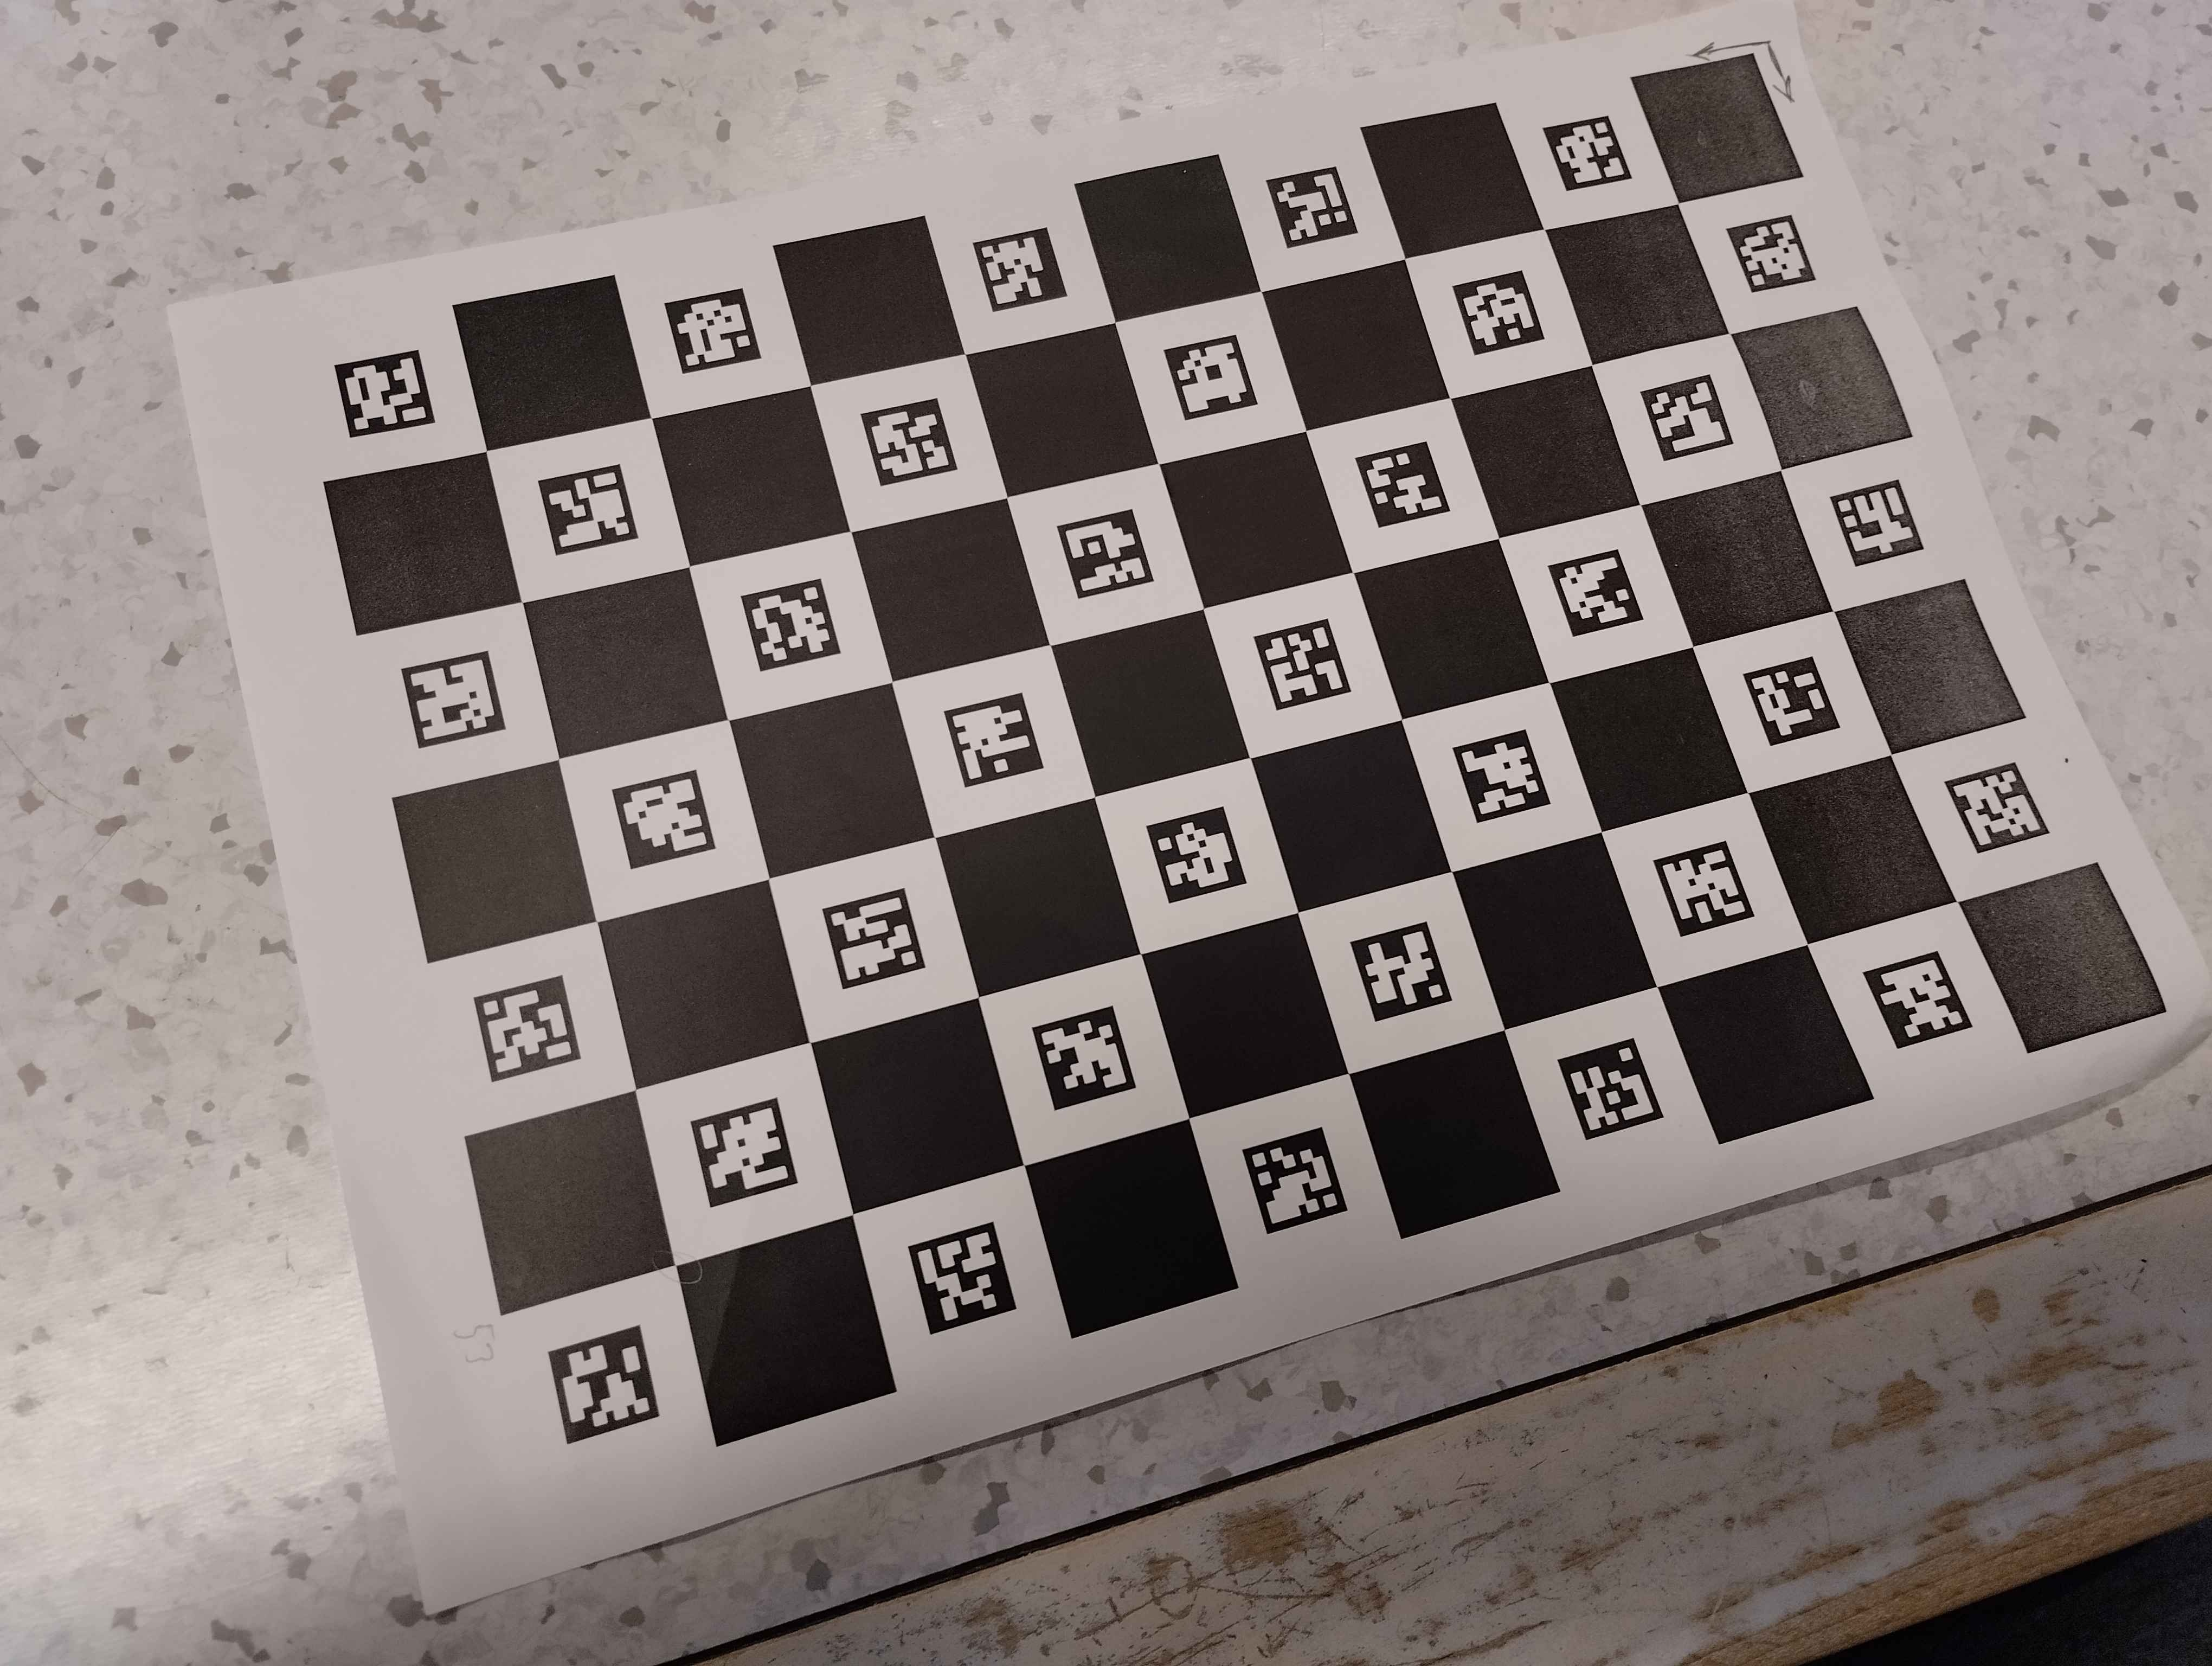
\includegraphics[width=.3\textwidth]{imgs/alphaorg.jpg}\hfill
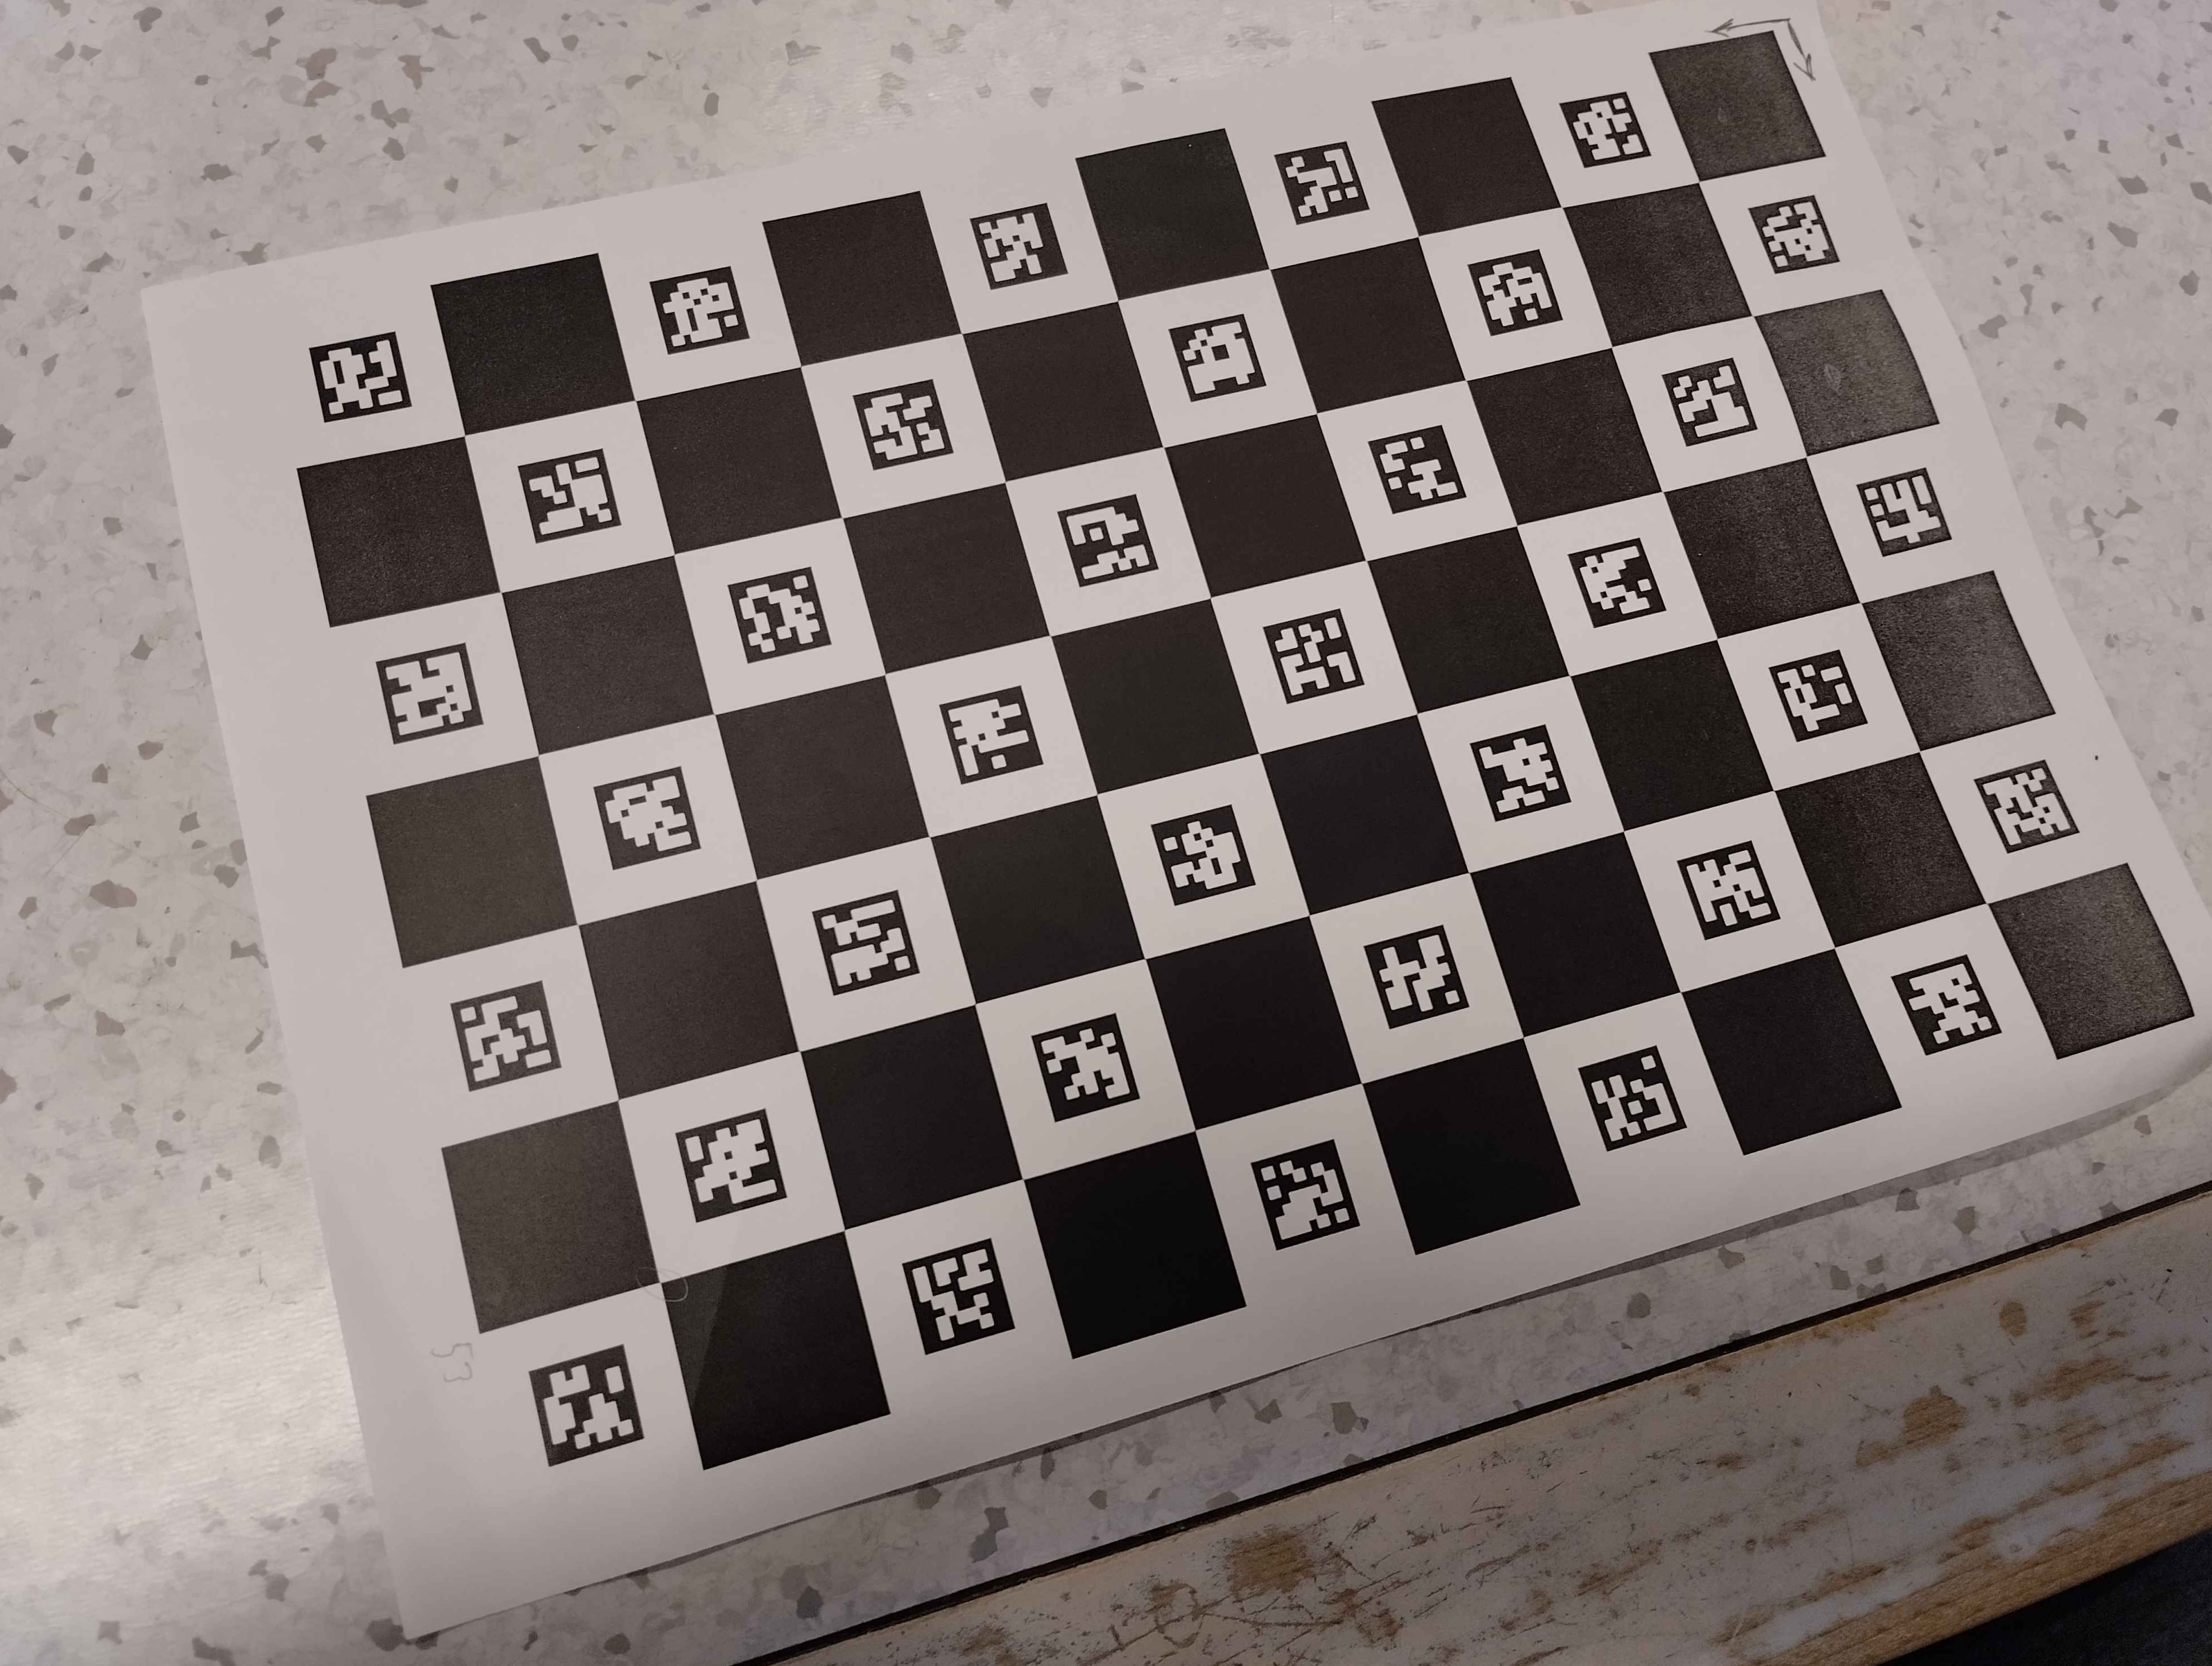
\includegraphics[width=.3\textwidth]{imgs/alpha0.jpg}\hfill
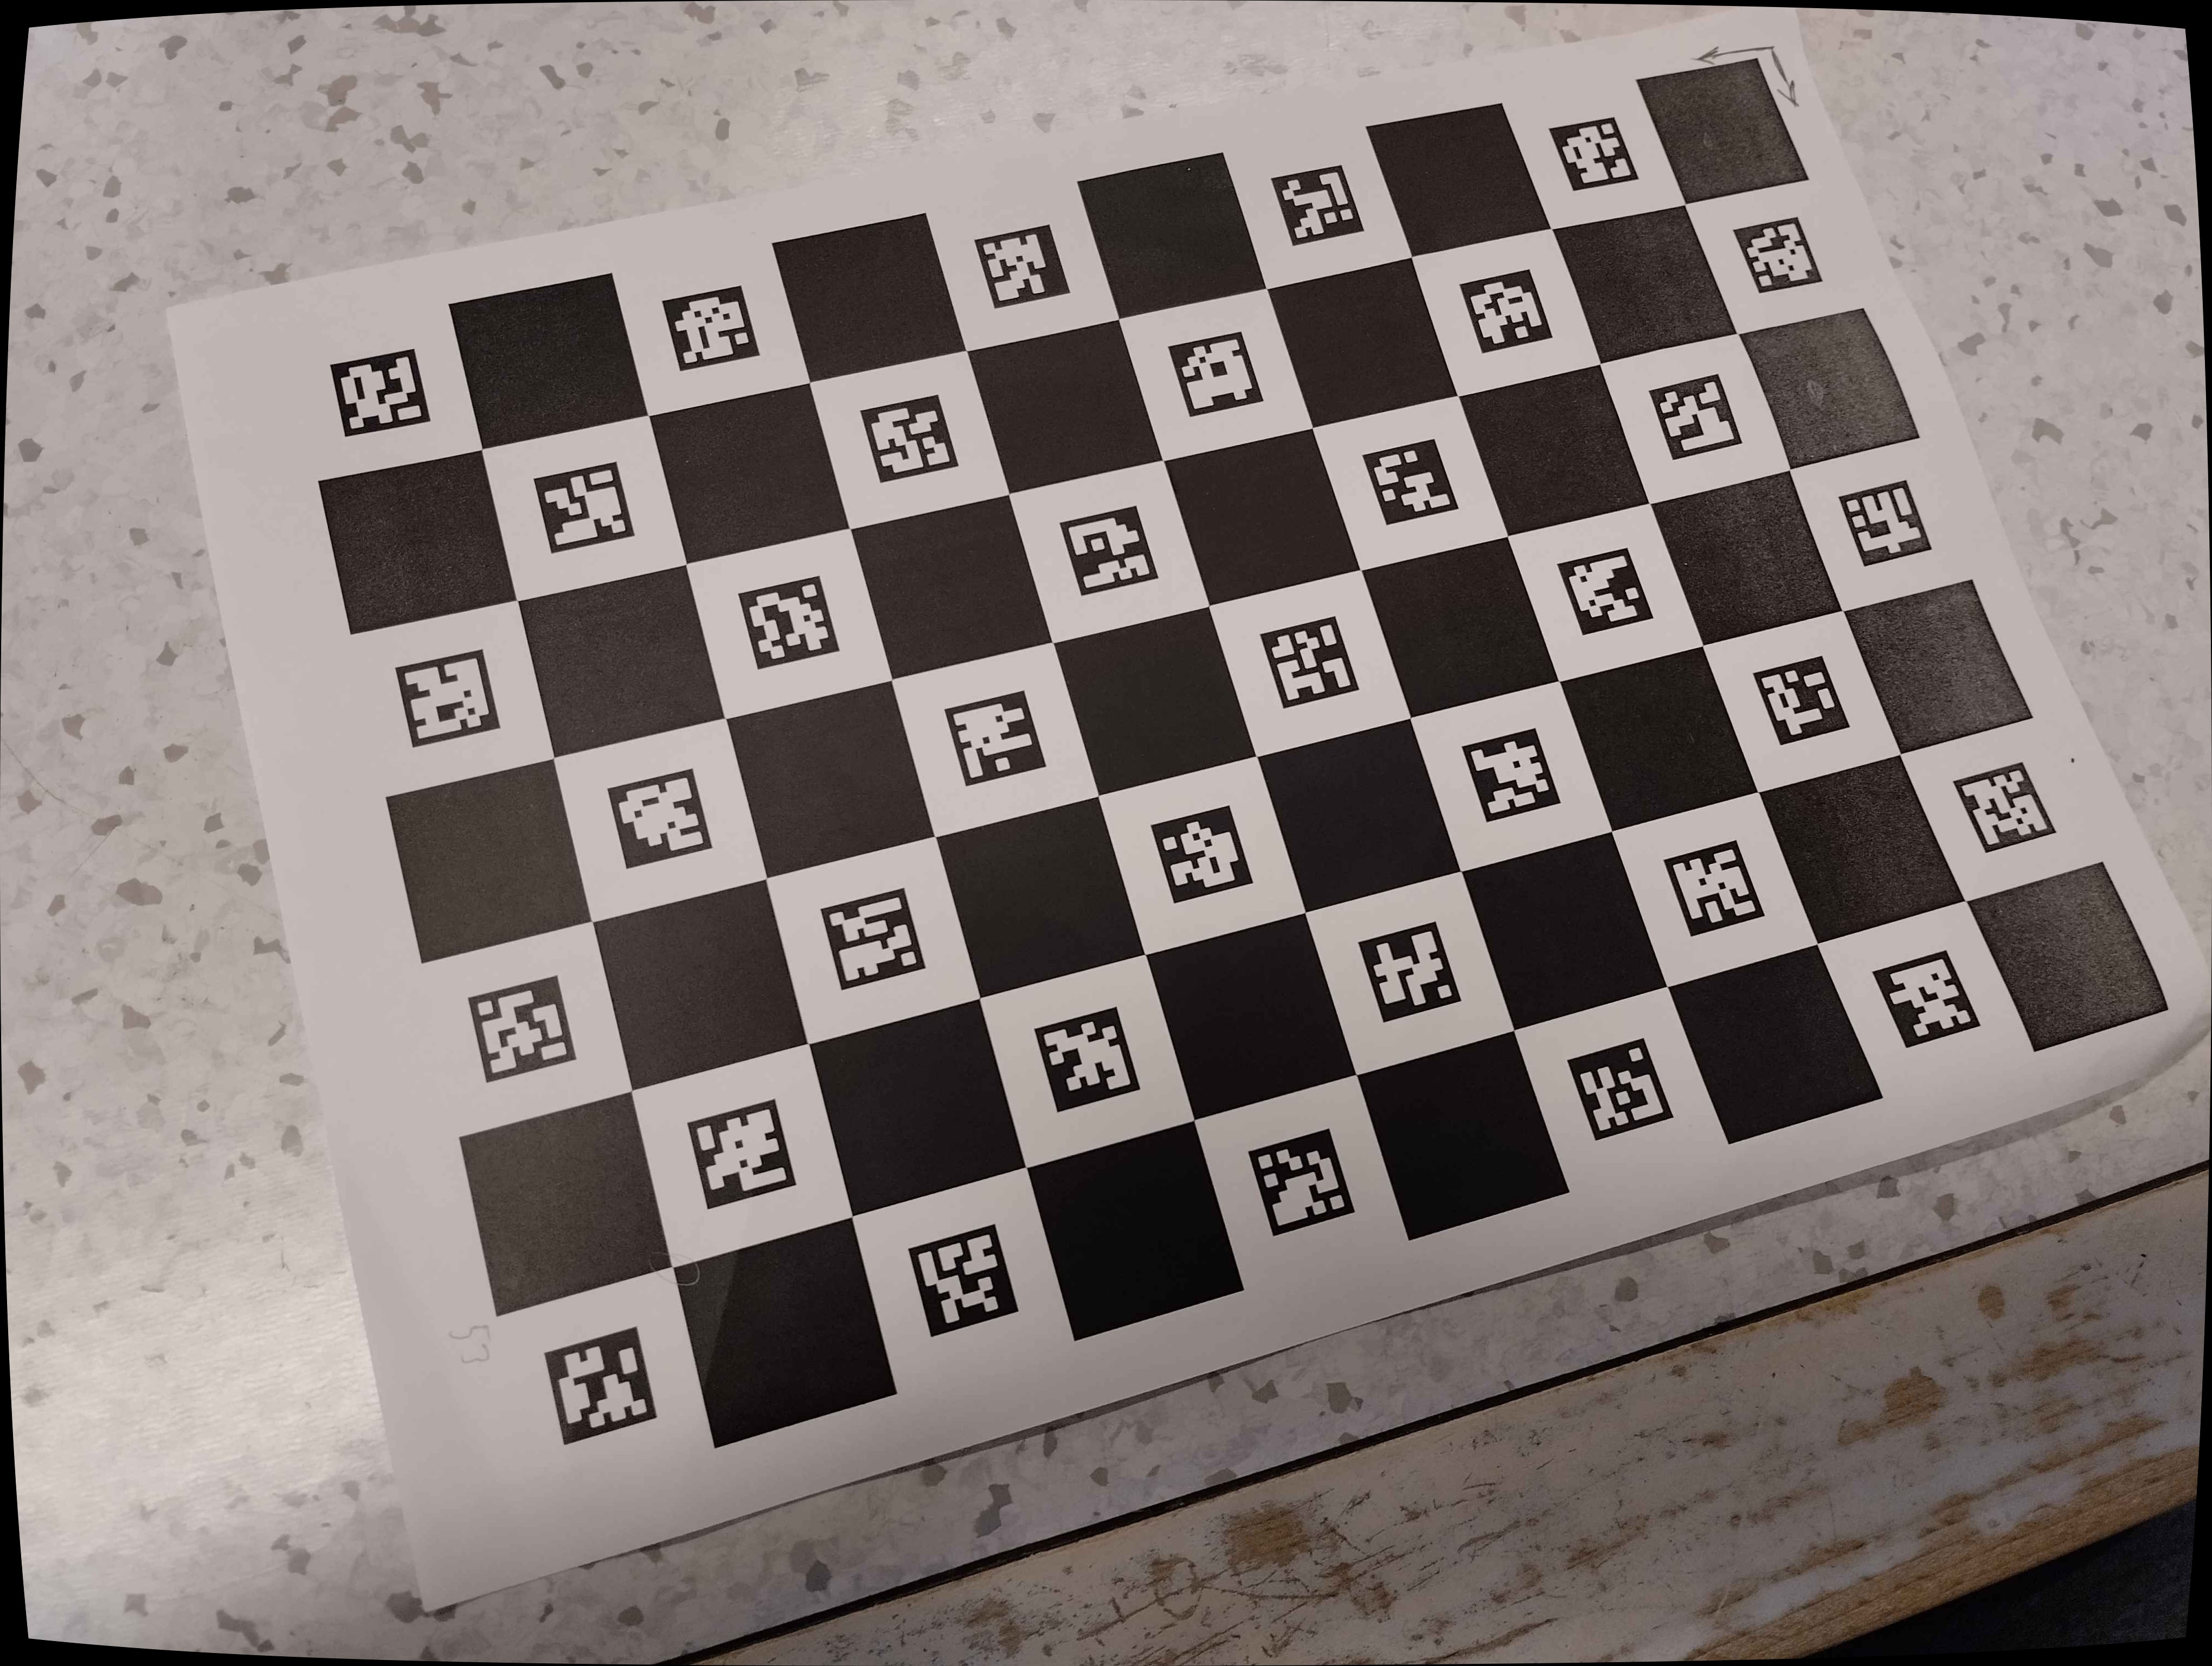
\includegraphics[width=.3\textwidth]{imgs/alpha1.jpg}

\caption{Results: a) original, b) alpha=0, c) alpha=1}
\label{fig:figure3}

\end{figure}

\section{Meshroom}
    Meshroom is a free, open-source 3D reconstruction software developed by AliceVision. The main way of using it is by connecting nodes which compute data. To start, open Meshroom, select File$\rightarrow$New Pipeline$\rightarrow$Photogrammetry, drag and drop the images of the object you want to reconstruct into the image gallery and press start. After the nodes have finished computing you can double click on them to view their results. 

\subsection{Nodes}

\subsubsection{CameraInit}
    This node processes the given pictures into data that Meshroom can use. It also reads the metadata from the pictures to acquire information that can be used later in the pipeline for example the focal length or the intrinsic parameters of the camera.


\subsubsection{FeatureExtraction}
    This node extracts distinct points from the images called features. In its parameters we can specify which method we can use. The default and a lot of the times the best method is dspsift(domain size pooling scale invariant feature transform), but there is also the akaze method which can be used for challenging surfaces like skin. Here we can also specify to extract points with cctags which we can use to scale the finished model by specifying the real world positions of those tags(Note: if using cctags, every picture must have at least 1 visible cctag and the pictures should be scaled down to something like 1920x1080 because it has a MAX\_RESOLUTION limit hard coded).
    In the settings of this node we can also give masks for the pictures so it only extracts points in a given field on the image. We can also change how much and the quality of the extracted points.
    
\subsubsection{ImageMatching}
    This node matches images so we know which images are close by so we can use them later for the FeatureMatching. There are multiple methods of ImageMatching. VocabularyTree sorting and comparing the extracted features of every image. Sequential matches images based on their name. Exhaustive matches every image with every image. Frustum matches based on the known image poses and matches images that are close by. 

\subsubsection{FeatureMatching}
    This node goes through the found image pairs and it finds similar features on both images. In the settings there is a parameter called minimal 2D motion. By default it is -1, meaning disabled, but if we put it to some positive value, like 2, we specify that a point to be matches, it needs to not be in the same position in both images. This option is useful to filter out background matches if we use turn tables because the background is static.

\subsubsection{StructureFromMotion}
    This node uses those matches features and uses that data to give us the position of those points in 3D space and the pose (position and orientation) and internal calibration of all the cameras. 

\subsubsection{PrepareDenseScene}
    This node undistorts the images. It uses the calibration parameters from the StructureFromMotion to compute the undistorted images. 

\subsubsection{DepthMap and DepthMapFilter}
    These nodes compute the depth maps of the images. The filter filters out incoherent depth map values. We can specify a downscale factor, the lower the factor is, the greater the quality, but the longer the computation time. We should use 1 only when we have very high quality images. 

\subsubsection{Meshing and MeshFiltering}
    Meshing is performed from the SfM data and the depth maps. The result is a dense geometric surface representation of the scene. This mesh then we can apply laplacian filtering to remove local defects. In the settings we can specify the output file type which we can find in the MeshroomCache folder and we can open and manipulate it with other applications like Blender.

\subsubsection{Texturing}
    This node textures the mesh. For each triangle, it uses the visibility information associated to each vertex to retrieve the texture candidates. It select the best cameras based on the resolution covering the triangle. Finally it averages the pixel values using multiple bands in the frequency domain. 

\subsection{Post processing}
    We can use an application like Blender to view and manipulate with our result mesh. Most commonly we can cut unwanted parts from our mesh, scale the mesh based on known geometry and then we can do measurements of the reconstructed object. 

\subsection{Results}
    To show the functionality of Meshroom, we will analyze the following reconstructions that i made and post-processed them in Blender.

    \subsubsection{Guitar}
    This model was made from 310 pictures from different angles. The guitar was positioned in the center of a desk and the desk was positioned in between 2 ceiling lamps so that the lighting is mostly equal from both sides. The pictures were taken by phone which i held. Because i held it and my hand isn't very stable i had to use a low shutter speed, 1/25s in these pictures, which made the pictures dark and to counter that i used a high ISO factor of 1200. I also put CCTags on the desk, but Meshroom gave me problems in scaling which i will fix in the future, and used them in Blender to scale the model. From the results we can see that a lot of my room was reconstructed from the backgrounds of the pictures, altho not in much detail. One of the things that Meshroom uses for matching is also background details, in this example that is great because every angle of the background is unique. I cut the guitar from the model in Blender. We can see that the neck of the guitar and the non glossy parts are very well reconstructed. The biggest mistake is in the body of the guitar. There is a big hole where the guitar is most glossy, that is because of the reflection of the lamps on the guitar body. In the future this can be removed by using a polarizing filter, using matte paint on the object or having better lighting. Also the pictures for this model were captured in JPG and in RAW format. The results for the reconstruction showed that JPG images were a lot better that those in RAW format. 
    
        \begin{figure}[h]
            \begin{subfigure}{.5\textwidth}
                \centering
                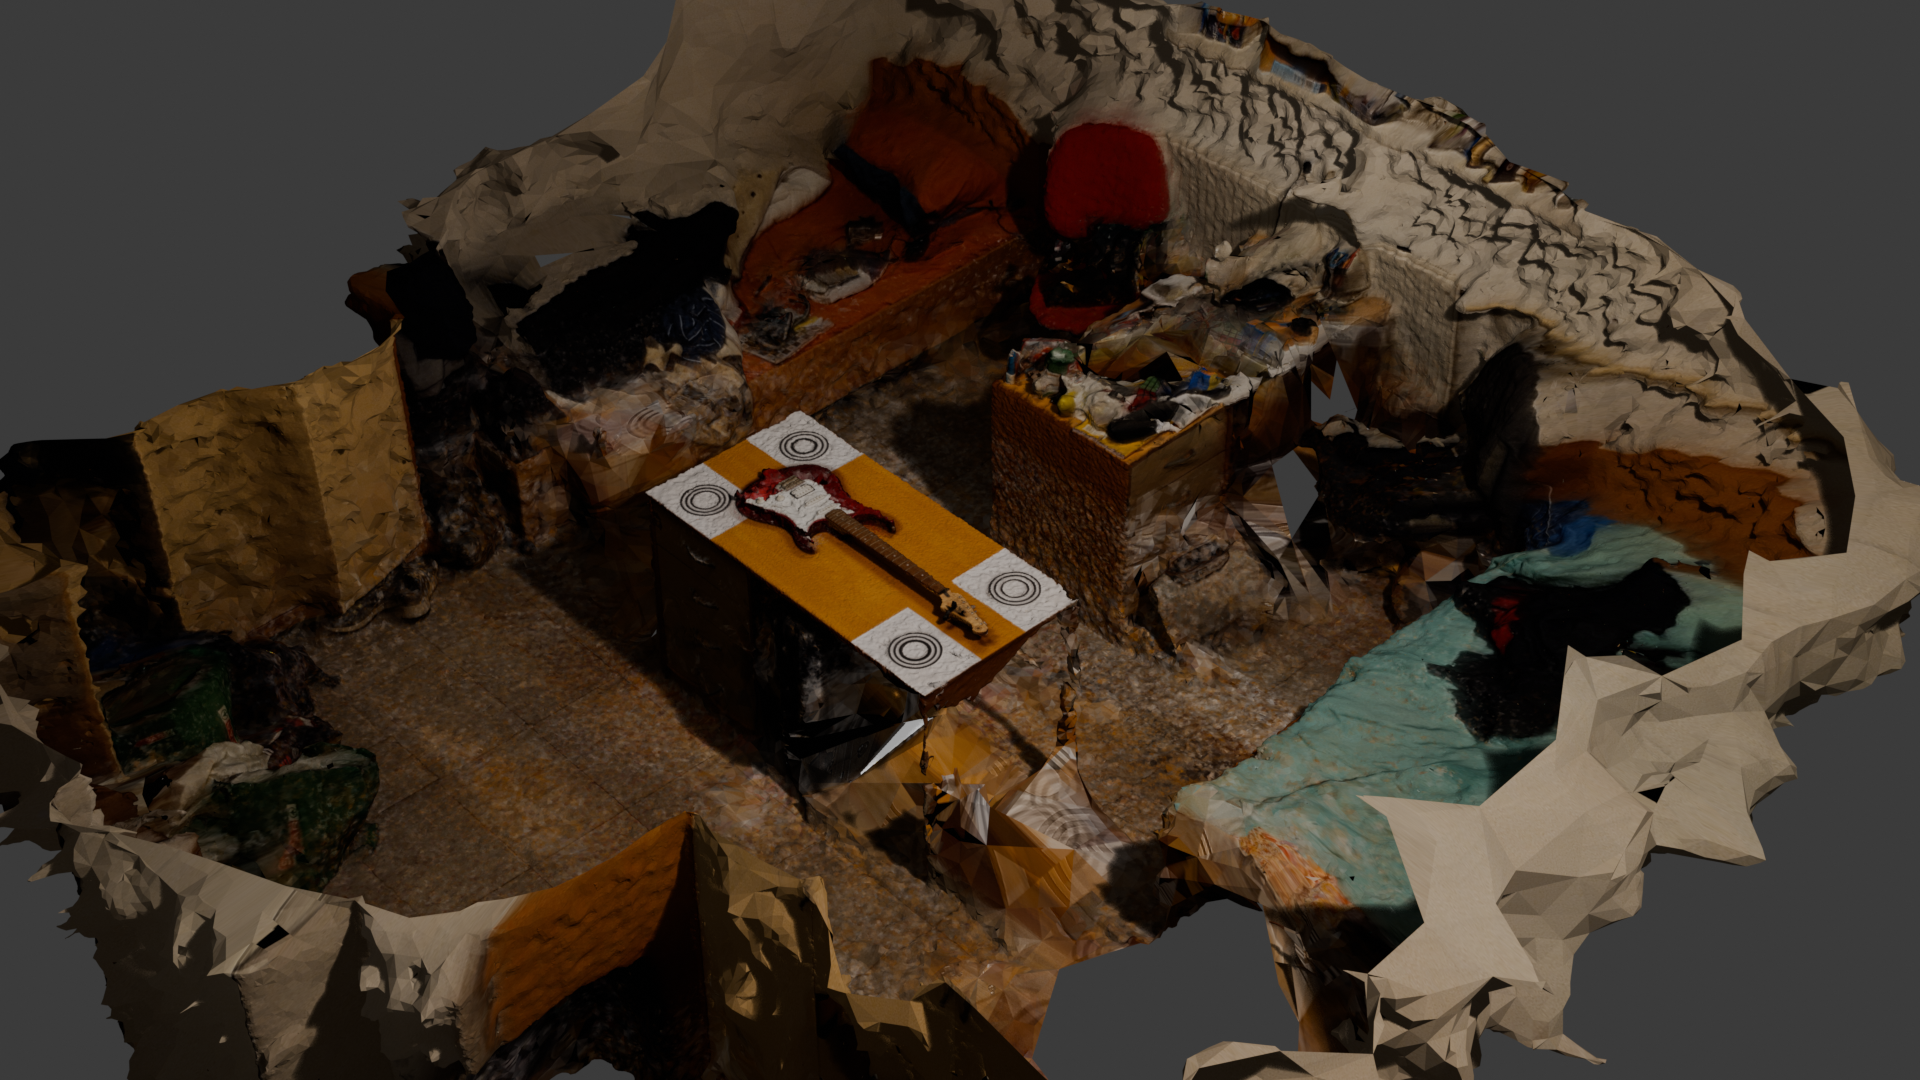
\includegraphics[width=.95\linewidth]{imgs/guitarsoba.png}
                \caption{Entire result from Meshroom}
            \end{subfigure}
            \begin{subfigure}{.5\textwidth}
                \centering
                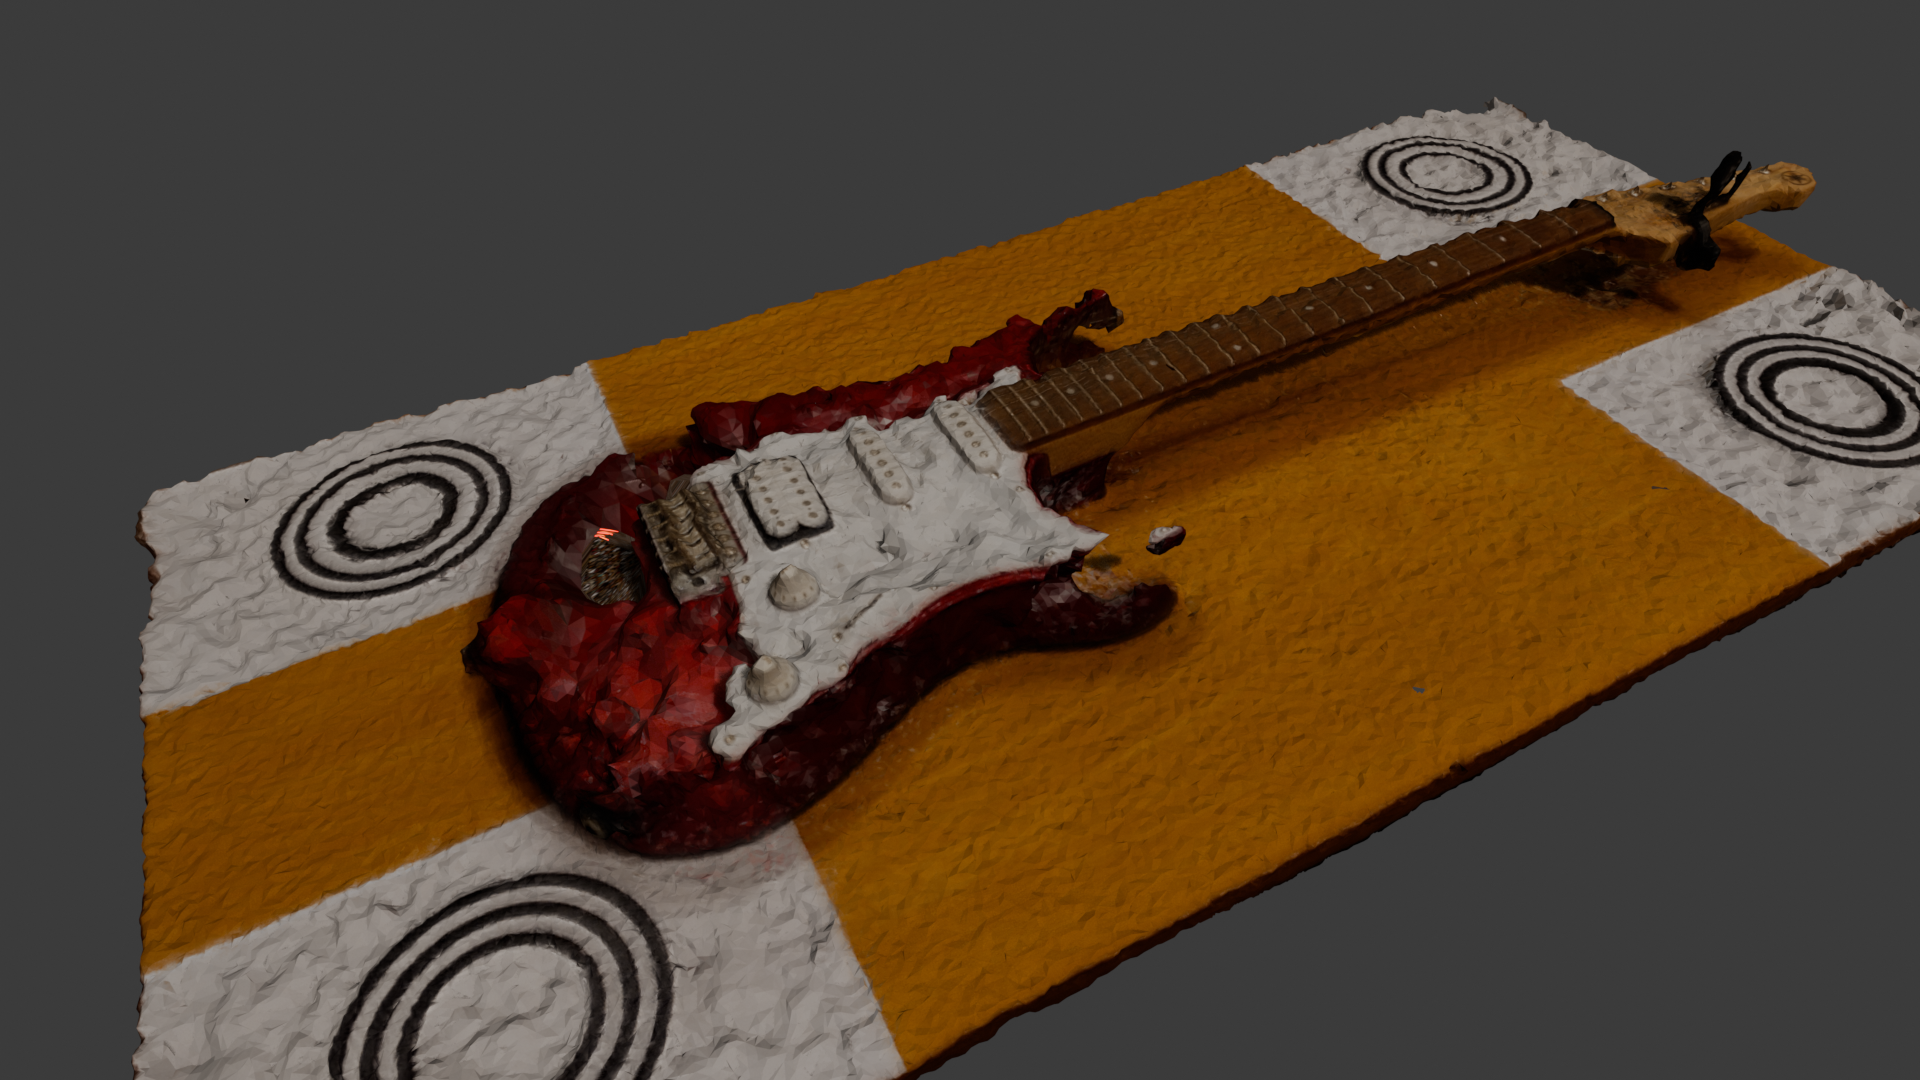
\includegraphics[width=.95\linewidth]{imgs/guitarcut.png}
                \caption{Cut result}
            \end{subfigure}
            \caption{Guitar reconstruction}
        \end{figure}
    
    \subsubsection{Eyelid}
        This model was made from 34 close up pictures of my black eye. The idea was to test how much detail can be captured on the face and the bruise. The lighting was from a desk lamp focused towards the eyelid. The shutter speed is 1/20s and the ISO is 150. The pictures were taken on a hand held phone. I did the reconstruction with different parameters so that they can be compared. The statistics on the objects can be seen in table \ref{tab:objstat}. We can see that for this example, dspsift is much better than akaze. We can also see that by having higher settings we get better results, but the difference between high and ultra is very small. From the bellow images we can notice that akaze has much more "waves" than dspsift.  

        \begin{table}[h]
            \centering
            \begin{tabular}{|c|c|c|c|c|c|} \hline 
                 &  DSPSift Normal&  DSPSift High&  DSPSift Ultra&  DSPSift+Akaze& Akaze\\ \hline 
                 Vertices&  319630&  325135&  325175&  324528& 151640\\ \hline 
                 Edges&  952816&  968875&  969452&  967321& 451475\\ \hline 
                 Faces&  635128&  645823&  646201&  644784& 300898\\ \hline
            \end{tabular}
            \caption{Object statistics}
            \label{tab:objstat}
        \end{table}

        \begin{figure}[h]
            \begin{subfigure}{.5\textwidth}
                \centering
                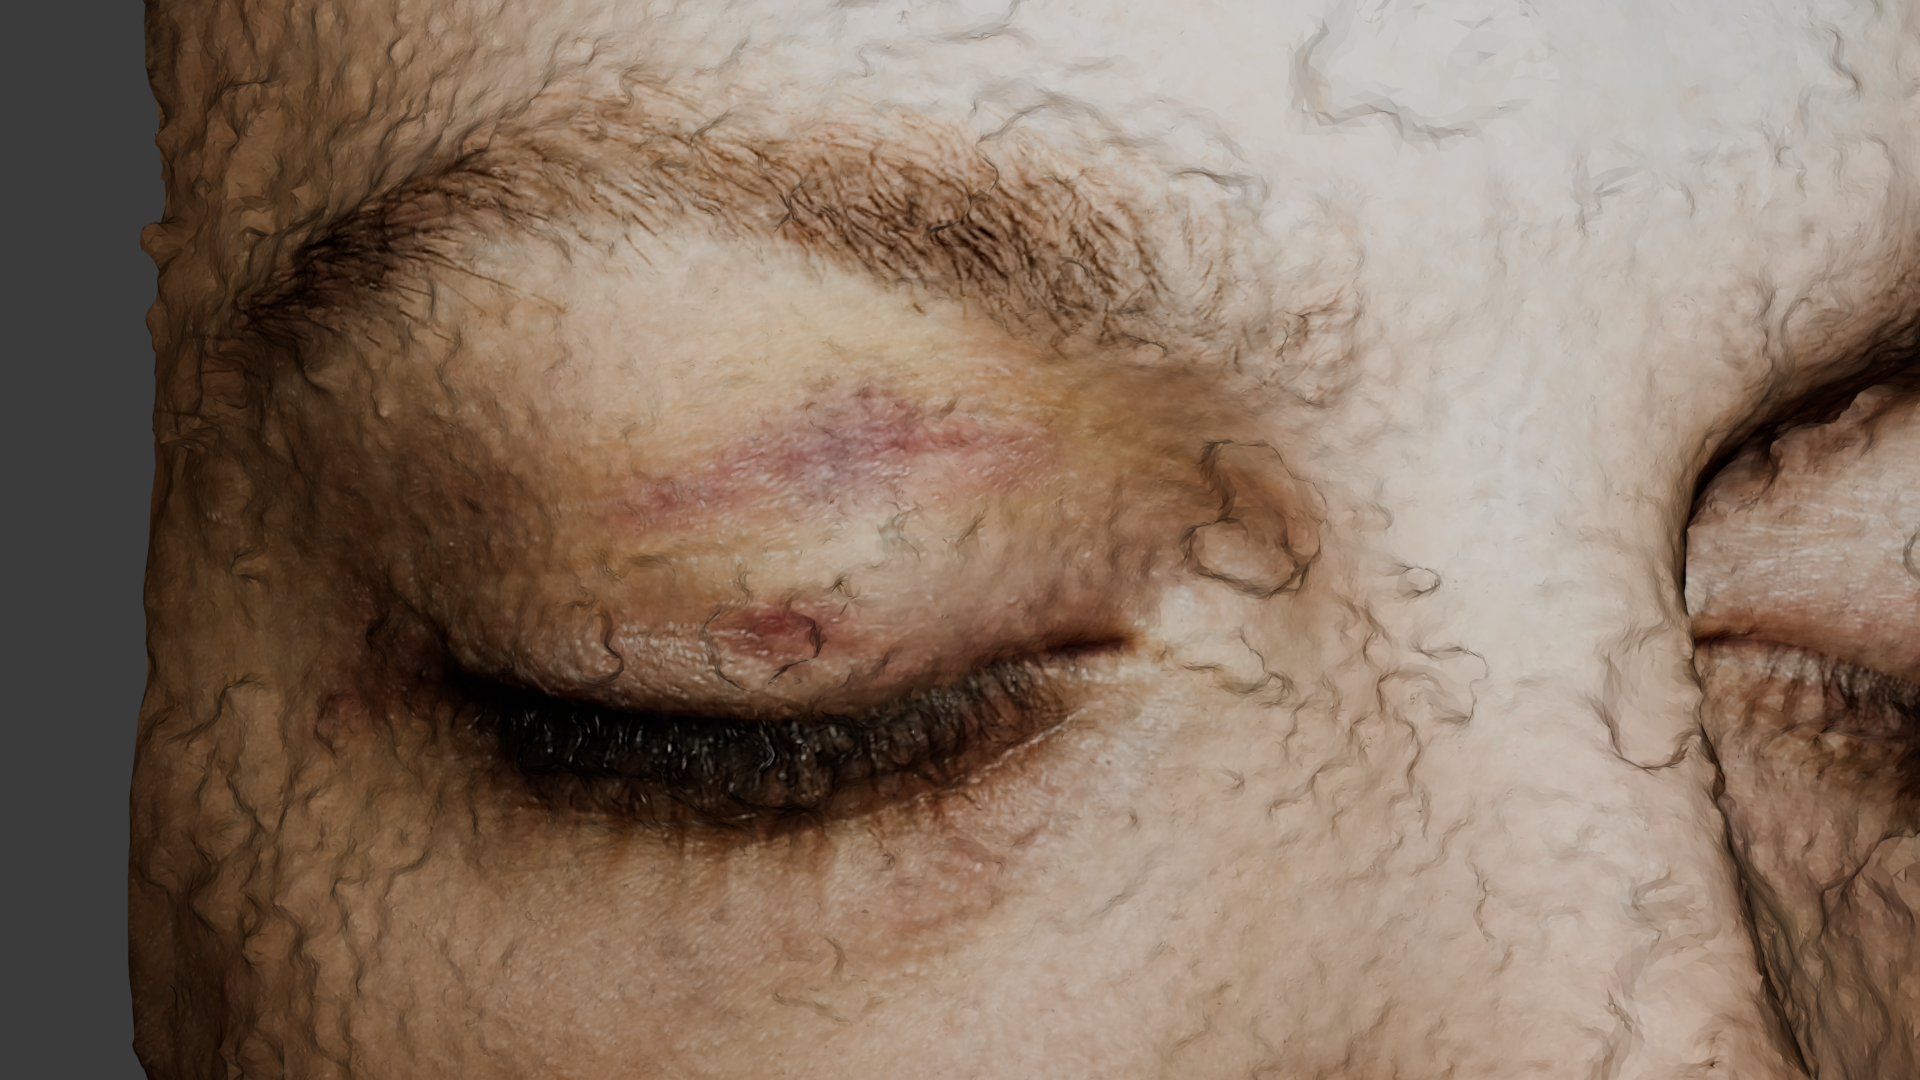
\includegraphics[width=.95\linewidth]{imgs/akaze.png}
                \caption{Akaze method}
            \end{subfigure}
            \begin{subfigure}{.5\textwidth}
                \centering
                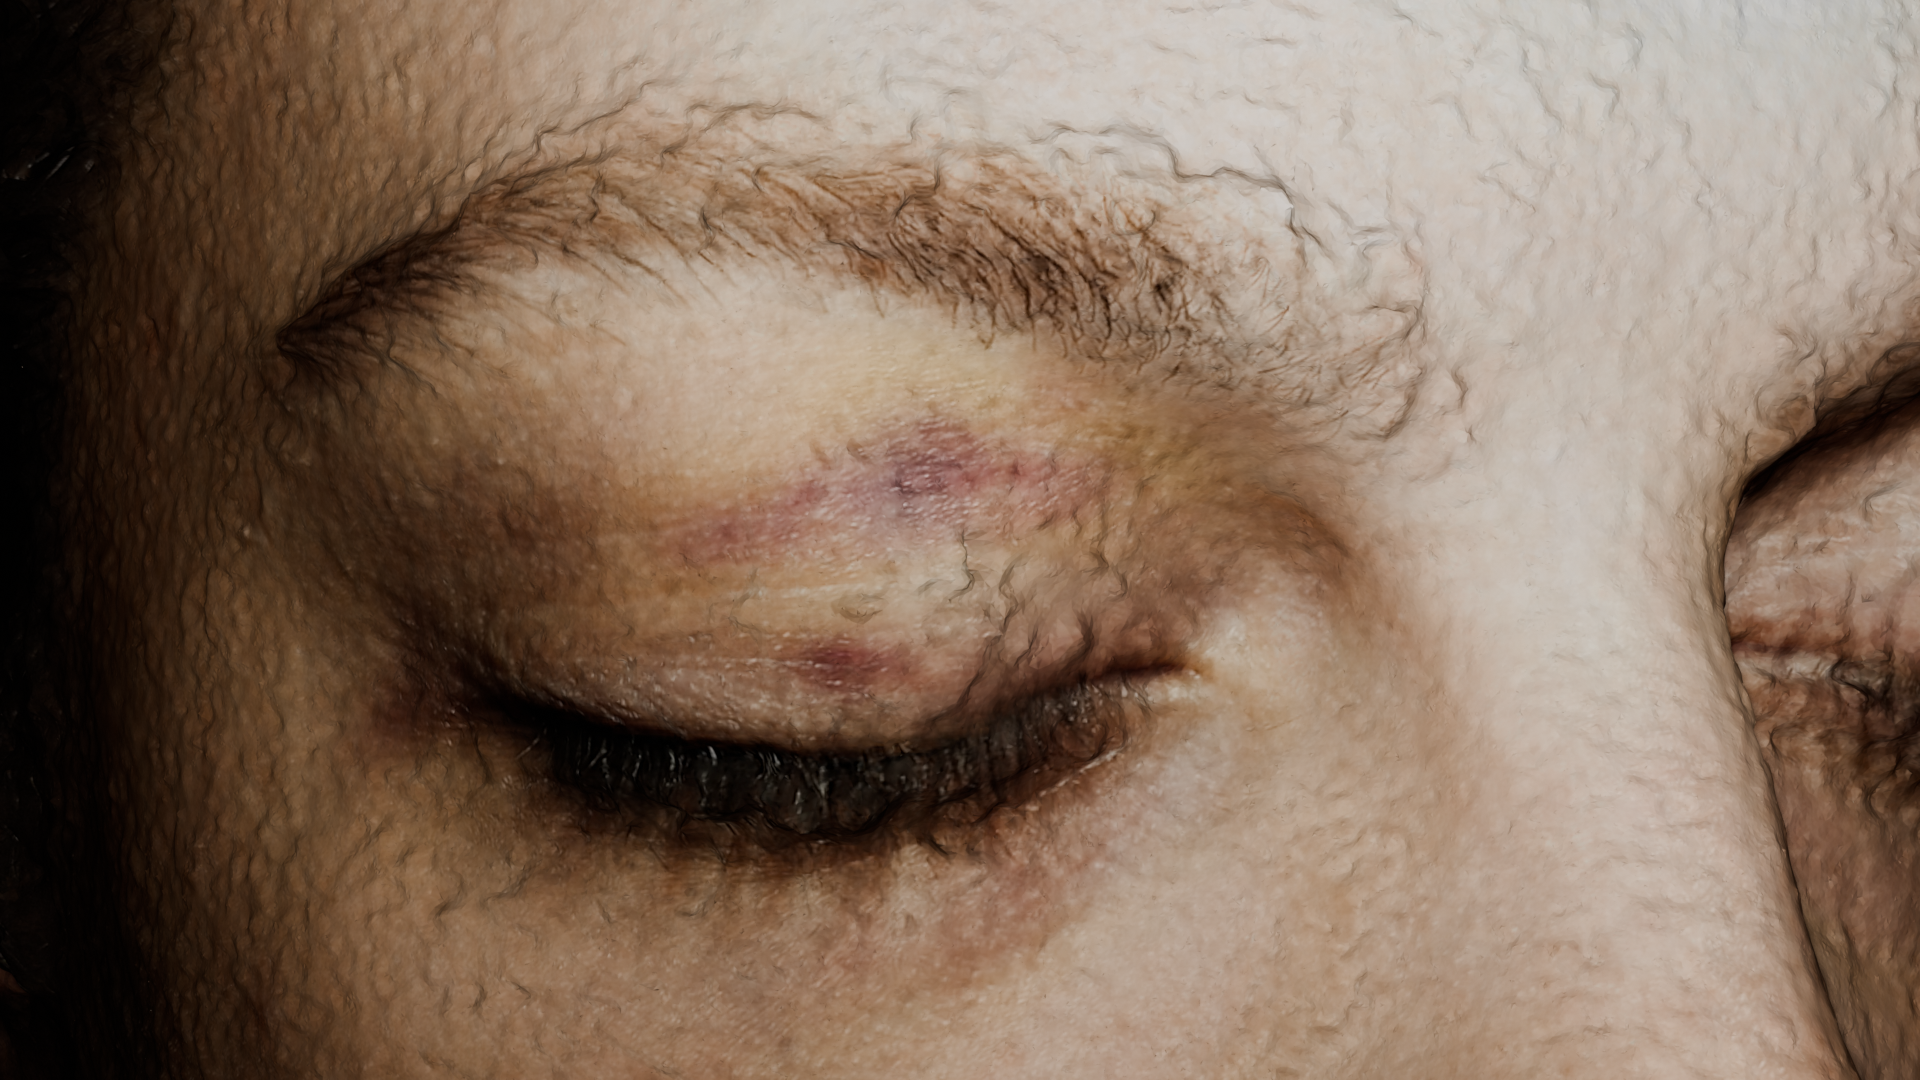
\includegraphics[width=.95\linewidth]{imgs/ultrarender.png}
                \caption{Ultra settings}
            \end{subfigure}
            \caption{Eyelid reconstruction}
        \end{figure}
    
    % \subsubsection{} %probaj parfem popravi ili arhitekt

    \subsubsection{Summary}
        For a good reconstruction we need to take good pictures. Ideally our camera should have a lower shutter speed and ISO factor. Also we should take our pictures in JPEG rather than RAW format. Lighting is very important. It should be directly on the object, not casting shadows. Out object should not be reflective because reflections of the light source give mistakes in the reconstructed model. DSPSift method for feature extraction is better than Akaze in the tested examples, but maybe for more difficult surfaces, Akaze might be appropriate. The settings on quality and quantity of extracted features should also be changed according to the number of images and the level of detail wanted. 
    
\end{document}
